\chapter{初等积分法}



\section{恰当方程}



\begin{exercise}
  判断下列方程是否为恰当方程; 并且对恰当方程求解.
  \begin{enumerate}[(1)]
  \item $(3x^2-1)\diff x+(2x+1)\diff y=0$.
  \item $(x+2y)\diff x+(2x-y)\diff y=0$.
  \item $(ax+by)\diff x+(bx+cy)\diff y=0$.
  \item $(ax-by)\diff x+(bx-cy)\diff y=0(b\neq0)$.
  \item $(t^2+1)\cos u\diff u+2t\sin u\diff t=0$.
  \item $(y\e^x+2\e^x+y^2)\diff x+(\e^x+2xy)\diff y=0$.
  \item $\displaystyle\left(\frac{y}{x}+x^2\right)\diff x+(\ln x-2y)\diff y=0$.
  \item $(ax^2+by^2)\diff x+cxy\diff y=0$.
  \item $\displaystyle\frac{2s-1}{t}\diff s+\frac{s-s^2}{t^2}\diff t=0$.
  \item $xf(x^2+y^2)\diff x+yf(x^2+y^2)\diff y=0$, 其中$f(\cdot)$是连续可微的.
  \end{enumerate}
\end{exercise}

\begin{solution}
	\begin{enumerate}[(1)]
		\item $\frac{\partial P}{\partial y}=0,\frac{\partial Q}{\partial x}=2$, 不是恰当方程.
		\item $\frac{\partial P}{\partial y}=2,\frac{\partial Q}{\partial x}=2$, 是恰当方程, 因为
			  \[(x+2y)\diff x+(2x-y)\diff y=\diff\left(\frac{1}{2}x^2+2xy-\frac{1}{2}y^2\right),\]
			  所以通积分为
			  \[\frac{1}{2}x^2+2xy-\frac{1}{2}y^2=C.\]
		\item $\frac{\partial P}{\partial y}=b=\frac{\partial Q}{\partial x}$, 是恰当方程, 因为
			  \[(ax+by)\diff x+(bx+cy)\diff y=\diff\left(\frac{1}{2}ax^2+bxy+\frac{1}{2}cy^2\right),\]
			  所以通积分为
			  \[\frac{1}{2}ax^2+bxy+\frac{1}{2}cy^2 = C.\]
		\item $\frac{\partial P}{\partial y}=-b\neq\frac{\partial Q}{\partial x}=b$, 不是恰当方程.
		\item $\frac{\partial P}{\partial t}=2t\cos u=\frac{\partial Q}{\partial u}$, 故是恰当方程, 因为
			  \[(t^2+1)\cos u\diff u+2t\sin u\diff t=\diff\left((t^2+1)\sin u\right),\]
			  所以通积分为
			  \[(t^2+1)\sin u = C.\]
		\item $\frac{\partial P}{\partial y}=\e^x+2y=\frac{\partial Q}{\partial x}$, 是恰当方程, 因为
			  \[(y\e^x+2\e^x+y^2)\diff x+(\e^x+2xy)\diff y=\diff(y\e^x+xy^2+2\e^x),\]
			  所以通积分为
			  \[y\e^x+xy^2+2\e^x = C.\]
		\item $\frac{\partial P}{\partial y}=\frac{1}{x}=\frac{\partial Q}{\partial x}$, 是恰当方程, 因为
			  \[\left(\frac{y}{x}+x^2\right)\diff x+(\ln x-2y)\diff y=\diff\left(y\ln x+\frac{1}{3}x^3-y^2\right),\]
			  所以通积分为
			  \[y\ln x+\frac{1}{3}x^3-y^2=C.\]
		\item $\frac{\partial P}{\partial y}=2by,\frac{\partial Q}{\partial x}=cy$, 
      因此当$2b=c$时方程为恰当方程, 此时
      \[(ax^2+by^2)\diff x+cxy\diff y=(ax^2+by^2)\diff x+2bxy\diff y
        = \diff\left(\frac{1}{3}ax^3+bxy^2\right),\]
      所以通积分为
      \[\frac{1}{3}ax^3+bxy^2 = C.\]
      当 $2b\neq c$ 时, 方程不是恰当方程.
		\item $\frac{\partial P}{\partial t}=\frac{1-2s}{t^2}=\frac{\partial Q}{\partial s}$, 
      是恰当方程, 因为
      \[\frac{2s-1}{t}\diff s+\frac{s-s^2}{t^2}\diff t=\diff\left(\frac{s^2-s}{t}\right),\]
      所以通积分为
      \[\frac{s^2-s}{t}=C.\]
		\item $\frac{\partial P}{\partial y}=2xyf'(x^2+y^2)=\frac{\partial Q}{\partial x}$, 
      是恰当方程, 且通积分为
			\[F(x^2+y^2)=C,\text{其中\ }F\text{\ 是\ }f\text{\ 的不定积分}.\qedhere\]
	\end{enumerate}
\end{solution}



\section{变量分离的方程}



\begin{exercise}
  求解下列微分方程, 并指出这些方程在$Oxy$平面上有意义的区域:
  \begin{enumerate}[(1)]
  \item $\displaystyle\frac{\diff y}{\diff x}=\frac{x^2}{y}$;
  \item $\displaystyle\frac{\diff y}{\diff x}=\frac{x^2}{y(1+x^3)}$;
  \item $\displaystyle\frac{\diff y}{\diff x}+y^2\sin x=0$;
  \item $\displaystyle\frac{\diff y}{\diff x}=1+x+y^2+xy^2$;
  \item $\displaystyle\frac{\diff y}{\diff x}=(\cos x\cos 2y)^2$;
  \item $\displaystyle x\frac{\diff y}{\diff x}=\sqrt{1-y^2}$;
  \item $\displaystyle\frac{\diff y}{\diff x}=\frac{x-\e^x}{y+\e^y}$.
  \end{enumerate}
\end{exercise}

\begin{solution}
  (1) $y^2=\frac{2}{3}x^3+C,y\neq 0$;

  (2) $y^2=\frac{2}{3}\ln|1+x^3|+C,y\neq0,x\neq-1$;

  (3) $\frac{1}{y}+\cos x=C$, 特解: $y=0$;

  (4) $y=\tan(x+\frac{1}{2}x^2+C)$;

  (5) 当 $\cos 2y\neq 0$ 时, 原方程等价于 $\frac{\diff y}{\cos^2 2y}=\sec^2 2y\diff y=\cos^2x\diff x$, 
  积分得 $2x+\sin2x-2\tan2y=C$, 当 $\cos2y=0$时, 有特解 $y=\frac{\pi}{4}+\frac{k\pi}{2}(k\in\mathbb{Z})$;

  (6) $\arcsin y=\ln|x|+C$, 特解: $y=\pm 1$;

  (7) $y^2-x^2+2(\e^y-\e^{-x})=C$ $(y+\e^y\neq 0)$.
\end{solution}



\begin{exercise}
  求解下列微分方程的初值问题:
  \begin{enumerate}[(1)]
  \item $\displaystyle\sin 2x\diff x+\cos 3y\diff y=0,\quad y\left(\frac{\pi}{2}\right)=\frac{\pi}{3}$;
  \item $\displaystyle x\diff x+y\e^{-x}\diff y=0,\quad y(0)=1$;
  \item $\displaystyle\frac{\diff r}{\diff\theta}=r,\quad r(0)=2$;
  \item $\displaystyle\frac{\diff y}{\diff x}=\frac{\ln|x|}{1+y^2},\quad y(1)=0$;
  \item $\displaystyle\sqrt{1+x^2}\frac{\diff y}{\diff x}=xy^3,\quad y(0)=1$.
  \end{enumerate}
\end{exercise}

\begin{solution}
  (1) 积分得 $-\frac{1}{2}\cos2x+\frac{1}{3}\sin3y+C=0$, 
  由 $y\left(\frac{\pi}{2}\right)=\frac{\pi}{3}$ 得 $C=-\frac{1}{2}$,
  因此原方程的解为 $2\sin3y-3\cos2x-3=0$.

  (2) 原方程等价于 $x\e^x\diff x+y\diff y=0$, 积分得 $(x-1)\e^x+\frac{1}{2}y^2+C=0$, 
  代入初值条件 $y(0)=1$ 得 $C=\frac{1}{2}$, 因此原方程的解为 $2(x-1)\e^x+y^2+1=0$.

  (3) 由初值条件知 $r\neq0$, 故 $\frac{\diff r}{r}=\diff\theta$, 积分得 $r=C\e^{\theta}$ $(C\neq 0)$,
  代入初值条件得 $C=2$, 因此原方程的解为 $r=2\e^{\theta}$.

  (4) $(1+y^2)\diff y=\ln|x|\diff x$, 积分得 $y+\frac{1}{3}y^3=x(\ln|x|-1)+C$, 
  代入初值条件得$C=1$, 因此原方程的解为 $y+\frac{1}{3}y^3=x(\ln|x|-1)+1$.

  (5) 由初值条件知 $y\neq 0$, 故原方程等价于 $\frac{\diff y}{y^3}=\frac{x}{\sqrt{1+x^2}}\diff x$, 
  积分得 $-\frac{1}{2}y^{-2}=\sqrt{1+x^2}+C$, 代入初值条件得 $C=-\frac{3}{2}$, 
  因此原方程的解为 $2\sqrt{1+x^2}+y^{-2}-3=0$.
\end{solution}



\begin{exercise}
  求解下列微分方程, 并作出相应积分曲线族的简图:
  \begin{enumerate}[(1)]
  \item $\displaystyle\frac{\diff y}{\diff x}=\cos x$;
  \item $\displaystyle\frac{\diff y}{\diff x}=ay$ $(a\neq 0\text{\ 为常数})$;
  \item $\displaystyle\frac{\diff y}{\diff x}=1-y^2$;
  \item $\displaystyle\frac{\diff y}{\diff x}=y^n$ $(n=\frac{1}{3},1,2)$.
  \end{enumerate}
\end{exercise}

\begin{solution}
  (1) $y=\sin x+C$, 积分曲线族如图~\ref{fig2.1}.
  \begin{figure}[htb]
    \centering
    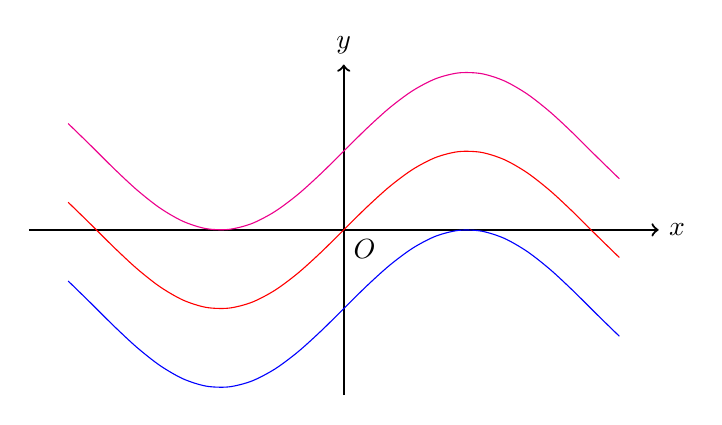
\begin{tikzpicture}[domain=-3.5:3.5]
    \draw[->,thick] (-4,0)--(4,0)node[anchor=west]{$x$};
    \draw[->,thick] (0,-2.1)--(0,2.1)node[anchor=south]{$y$};
    \draw (0,0)node[anchor=north west]{$O$};
    \draw[color=red,smooth] plot(\x,{sin(\x r)});
    \draw[color=blue,smooth]plot(\x,{sin(\x r)-1});
    \draw[color=magenta,smooth]plot(\x,{sin(\x r)+1});
    \end{tikzpicture}
    \caption{$y=\sin x+C$}
    \label{fig2.1}
  \end{figure}

  (2) $y=0$为特解, 当 $y\neq 0$ 时, 积分得$y=C\e^{ax}$ $(C\neq 0)$, 
  积分曲线族如图~\ref{fig2.2} (以 $a>0$ 为例).
  \begin{figure}
    \centering
    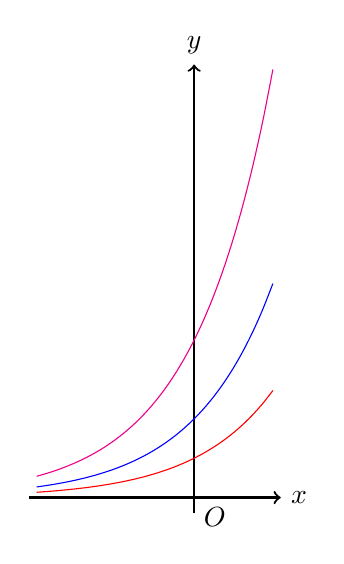
\begin{tikzpicture}[domain=-2:1]
    \draw[->,thick] (-2.1,0)--(1.1,0)node[anchor=west]{$x$};
    \draw[->,thick] (0,-0.2)--(0,5.5)node[anchor=south]{$y$};
    \draw (0,0)node[anchor=north west]{$O$};
    \draw[color=red,smooth]plot(\x,{0.5*exp(\x)});
    \draw[color=blue,smooth]plot(\x,{exp(\x)});
    \draw[color=magenta,smooth]plot(\x,{2*exp(\x)});
    \end{tikzpicture}
    \caption{$y=C\e^{ax}$}
    \label{fig2.2}
  \end{figure}

  (3) $y=\pm1$为特解, 当 $y\neq\pm 1$ 时, $\frac{\diff y}{1-y^2}=\diff x$, 
  积分得 $y=\frac{C\e^{2x}-1}{C\e^{2x}+1}(C\neq0)$, 
  当$C>0$时, 函数图像位于直线 $y=1$ 和 $y=-1$ 之间且单调递增; 
  当$C<0$时, 存在间断点 $x_0=\frac{1}{2}\ln\left(-\frac{1}{C}\right)$, 
  $y=y(x)$ 在 $(-\infty,x_0)$ 上单调递减且当 $x\to x_0-$ 时 $y\to-\infty$, 
  在 $(x_0,\infty)$ 上单调递减且当 $x\to x_0+$ 时 $y\to+\infty$, 积分曲线族如图~\ref{fig2.3}.
  \begin{figure}
    \centering
    \begin{tikzpicture}[domain=-3.5:3.5]
      \draw[->,thick] (-4,0)--(4,0)node[anchor=west]{$x$};
      \draw[->,thick] (0,-5)--(0,6)node[anchor=south]{$y$};
      \draw(0,0)node[anchor=south east]{$O$};
      \draw[color=yellow,smooth]plot(\x,1);
      \draw[color=yellow,smooth]plot(\x,-1);
      \draw(-2,1)node[anchor=south]{$y=1$};
      \draw(2,-1)node[anchor=south]{$y=-1$};
      \draw[dashed](0.3466,-5)--(0.3466,6);
      \draw(0.3466,-2)node[anchor=west]{$x=\frac{1}{2}\ln\left(-\frac{1}{C}\right)(C<0)$};
      \draw[color=red,smooth]plot(\x,{(exp(2*\x)-1)/(exp(2*\x)+1)});
      \draw[color=red,smooth]plot(\x,{(2*exp(2*\x)-1)/(2*exp(2*\x)+1)});
      \draw[color=red,smooth]plot(\x,{(0.5*exp(2*\x)-1)/(0.5*exp(2*\x)+1)});
      \draw[color=red,smooth]plot(\x,{(exp(2*\x)-1)/(exp(2*\x)+1)});
      \draw[color=blue,smooth,domain=-3.5:0.15]plot(\x,{(-0.5*exp(2*\x)-1)/(-0.5*exp(2*\x)+1)});
      \draw[color=blue,smooth,domain=0.55:3.5]plot(\x,{(-0.5*exp(2*\x)-1)/(-0.5*exp(2*\x)+1)});
    \end{tikzpicture}
  \caption{$y=\pm 1$和$y=\frac{C\e^{2x}-1}{C\e^{2x}+1}$}
  \label{fig2.3}
  \end{figure}

  (4) 下述三种情形积分曲线族都易作出(略去).
  \begin{enumerate}[(i)]
  \item $n=\frac{1}{3}$ 时, 通解为 $\frac{3}{2}y^{\frac{2}{3}}=x+C$ $(x\geq-C)$, 特解为 $y=0$;
  \item $n=1$时, 通解为 $y=C\e^x$ $(C\in\mathbb{R})$;
  \item $n=2$时, 通解为 $y=\frac{1}{-x+C}$ $(C\in\mathbb{R})$, 特解为$y=0$.
  \end{enumerate}
\end{solution}



\begin{exercise}
  跟踪: 设某 $A$ 从 $Oxy$ 平面上的原点出发, 沿 $x$ 轴正方向前进; 同时某 $B$ 从点 $(0,b)$ 开始跟踪 $A$, 
  即 $B$ 的运动方向永远指向 $A$ 并与 $A$ 保持等距 $b$. 试求 $B$ 的光滑运动轨迹.
\end{exercise}

\begin{solution}
  设 $B$ 的运动轨迹方程为 $y=y(x)$, 记某时刻 $B$ 的位置为 $(x,y(x))$, 
  则此时 $A$ 相应的位置为 $\left(x-\frac{y(x)}{y'(x)},0\right)$, 由于 $A$ 与 $B$ 保持等距, 故
  \[\left(\frac{y}{y'}\right)^2+y^2=b^2\Rightarrow\diff x=-\frac{\sqrt{b^2-y^2}}{y}\diff y.\]
  积分得
  \[\begin{split}
  x
  & = -\int\frac{\sqrt{b^2-y^2}}{y}\diff y(y=b\cos\theta) \\
  & = -\int\frac{b\sin\theta}{b\cos\theta}(-b\sin\theta)\diff\theta \\
  & = b\int(\sec\theta-\cos\theta)\diff\theta \\
  & = b\ln|\sec\theta+\tan\theta|-b\sin\theta+C \\
  & = b\ln\frac{b+\sqrt{b^2-y^2}}{y}-\sqrt{b^2-y^2}+C.
  \end{split}\]
  由初值条件 $y(0)=b$ 得 $C=0$, 故 $B$ 的光滑运动轨迹方程为
  $x=b\ln\frac{b+\sqrt{b^2-y^2}}{y}-\sqrt{b^2-y^2}$.
\end{solution}



\begin{exercise}
  设微分方程
  \[\frac{\diff y}{\diff x}=f(y),\]
  其中 $f(y)$ 在 $y=a$ 的某邻域 (例如区间 $|y-a|\leq\varepsilon$) 内连续, 而且$f(y)=0$当且仅当$y=a$. 
  证明: 在直线$y=a$上的每一点, 上述方程的解是局部唯一的, 当且仅当瑕积分
  \[\left|\int_a^{a\pm\varepsilon}\frac{\diff y}{f(y)}\right|=\infty.\]
\end{exercise}

\begin{solution}
  ($\Leftarrow$) 显然, $y=a$ 是方程的一个解, 用反证法, 设 $y=y(x)$ 是方程的另一个解, 
  它与直线 $y=a$ 相交. 不妨设 $(x_0,a)$ 是它们的一个交点, 
  且存在区间 $I=(x_0,x_0+\delta)$ 或 $I=(x_0-\delta,x_0)$, 
  使得当 $x\in I$ 时, $y(x)\neq a$, 从而
  \[\frac{\diff y(x)}{f(y(x))}=\diff x,\quad x\in I.\]
  积分得
  \[\int_a^y\frac{\diff y}{f(y)}=\int_{x_0}^x\frac{\diff y(x)}{f(y(x))}
    = \int_{x_0}^x\diff x = x-x_0<\infty.\]
  矛盾.

  $(\Rightarrow)$ 用反证法, 设 $\left|\int_a^{a\pm\varepsilon}\frac{\diff y}{f(y)}\right|<+\infty$,
  则由
  \[\int_a^y\frac{\diff y}{f(y)}=x-x_0\]
  定义的函数是方程的解, 且通过点 $(x_0,a)$, 而 $y=a$ 也是过点 $(x_0,a)$ 的解, 矛盾.
\end{solution}



\begin{exercise}
  利用上题结果,作出下列微分方程积分曲线族的草图:
  \[(1)\frac{\diff y}{\diff x}=\sqrt{|y|};\quad
  (2)\frac{\diff y}{\diff x}=
  \begin{cases}
    y\ln|y|, & y\neq 0, \\
    0,       & y=0.
  \end{cases}\]
\end{exercise}

\begin{solution}
(1) 因为 $\int_0^{\pm\varepsilon}\frac{\diff y}{\sqrt{|y|}}$ 收敛, 故解不是局部唯一的, 微分方程的通解为
\[y=
  \begin{cases}
    \frac{1}{4}(x+C)^2,  & x\geq -C, \\
    -\frac{1}{4}(x+C)^2, & x\leq -C.
  \end{cases}\]
另外特解为 $y=0$, 积分曲线族容易作出.

(2) 因为 $\int_0^{\pm\varepsilon}\frac{\diff y}{y\ln|y|}$ 发散, 所以解是局部唯一的, 微分方程的通解为
\[y=\pm\e^{C\e^x}\quad(C\in\mathbb{R}).\]
另外特解为 $y=0$, 积分曲线族容易作出.
\end{solution}



\section{一阶线性方程}



\begin{exercise}
  求解微分方程:
  \begin{enumerate}[(1)]
  \item $\displaystyle\frac{\diff y}{\diff x}+2y=x\e^{-x}$;
  \item $\displaystyle\frac{\diff y}{\diff x}+y\tan x=\sin(2x)$;
  \item $\displaystyle x\frac{\diff y}{\diff x}+2y=\sin x$, $y(\pi)=\frac{1}{\pi}$;
  \item $\displaystyle\frac{\diff y}{\diff x}-\frac{1}{1-x^2}y=1+x$, $y(0)=1$.
  \end{enumerate}
\end{exercise}

\begin{solution}
  (1) $p(x)=2$, $q(x)=x\e^{-x}$, 故
  \[y=\e^{-\int2\diff x}\left(C+\int x\e^{-x}\e^{\int2\diff x}\diff x\right)=C\e^{-2x}+(x-1)\e^{-x}.\]

  (2) $p(x)=\tan x$, $q(x)=\sin(2x)$, 故
  \[\begin{split}
  y
  & = \e^{-\int\tan x\diff x}\left(C+\int\sin(2x)\e^{\int\tan x\diff x}\diff x\right)\\
  & = |\cos x|\left(C+\int\frac{\sin(2x)}{|\cos x|}\diff x\right)=C|\cos x|-2\cos^2x。
  \end{split}\]

  (3) $p(x)=\frac{2}{x}$, $q(x)=\frac{\sin x}{x}$, 故
  \[y=\e^{-\int\frac{2}{x}\diff x}\left(C+\int\frac{\sin x}{x}\e^{\int\frac{2}{x}\diff x}\diff x\right)=\frac{1}{x^2}(C+\sin x-x\cos x).\]
  代入初值条件得 $C=0$, 故原方程的解为
  \[y=\frac{\sin x}{x^2}-\frac{\cos x}{x}.\]

  (4) $p(x) = -\frac{1}{1-x^2}$, $q(x)=1+x$, 故
  \begin{align*}
    y
    & = \e^{\int\frac{1}{1-x^2}\diff x}\left(C+\int(1+x)\e^{\int\frac{1}{x^2-1}\diff x}\diff x\right) \\
    & = \left|\frac{x+1}{x-1}\right|^{\frac{1}{2}}\left(C+\int(1+x)\left|\frac{x-1}{x+1}\right|^{\frac{1}{2}}\diff x\right)\\
    & = \begin{cases}
      \sqrt{\frac{x+1}{x-1}}\left(C+\int\sqrt{x^2-1}\diff x\right), & |x|>1, \\
      \sqrt{\frac{x+1}{1-x}}\left(C+\int\sqrt{1-x^2}\diff x\right), & |x|<1,
    \end{cases} \\
    & = \begin{cases}
      \sqrt{\frac{x+1}{x-1}}\left(C+\frac{1}{2}x\sqrt{x^2-1}-\frac{1}{2}\ln|x+\sqrt{x^2-1}|\right),
        & |x|>1, \\
        \sqrt{\frac{x+1}{1-x}}\left(C+\frac{1}{2}\arcsin x+\frac{1}{2}x\sqrt{1-x^2}\right),
        & |x|<1.
    \end{cases}\qedhere
  \end{align*}
\end{solution}



\begin{exercise}
  把下列微分方程化为线性微分方程:
  \begin{enumerate}[(1)]
  \item $\displaystyle\frac{\diff y}{\diff x}=\frac{x^2+y^2}{2y}$;
  \item $\displaystyle\frac{\diff y}{\diff x}=\frac{y}{x+y^2}$;
  \item $\displaystyle 3xy^2\frac{\diff y}{\diff x}+y^3+x^3=0$;
  \item $\displaystyle\frac{\diff y}{\diff x}=\frac{1}{\cos y}+x\tan y$.
  \end{enumerate}
\end{exercise}

\begin{solution}
  (1) 令 $u=y^2$, 则 $\frac{\diff u}{\diff x}=2y\frac{\diff y}{\diff x}=x^2+u$.

  (2) 将 $x$ 看作 $y$ 的函数, 即 $\frac{\diff x}{\diff y}=\frac{x}{y}+y$.

  (3) 令 $u=y^3$, 则 $\frac{\diff u}{\diff x}=3y^2\frac{\diff y}{\diff x}=-\frac{u}{x}-x^2$.

  (4) 原方程变形为 $\cos y\frac{\diff y}{\diff x}=1+x\sin y$,
  令 $u=\sin y$, 即得 $\frac{\diff u}{\diff x}=1+xu$.
\end{solution}



\begin{exercise}
  设 $y=\varphi(x)$ 满足微分不等式
  \[y'+a(x)y\leq 0\quad (x\geq 0).\]
  求证:
  \[\varphi(x)\leq\varphi(0)\e^{-\int_0^x a(s)\diff s}\quad (x\geq 0).\]
\end{exercise}

\begin{proof} 
在不等式两边同时乘以 $\e^{\int_0^xa(s)\diff s}$, 得
\[\e^{\int_0^xa(s)\diff s}\frac{\diff y}{\diff x}+a(x)y\e^{\int_0^xa(s)\diff s}\leq 0,\]
即
\[\frac{\diff\left(\varphi(x)\e^{\int_0^xa(s)\diff s}\right)}{\diff x}\leq 0.\]
将上式从 $0$ 到 $x$ 积分得
\[\varphi(x)\e^{\int_0^xa(s)\diff s}-\varphi(0)\leq 0
\Rightarrow\varphi(x)\leq\varphi(0)\e^{-\int_0^xa(s)\diff s}.\qedhere\]
\end{proof}



\begin{exercise}
  用常数变易法求解非齐次线性方程 $\frac{\diff y}{\diff x}+p(x)y=q(x)$, 即: 
  假设方程有形如 $y=C\e^{-\int p(x)\diff x}$ 的解, 但其中的常数 $C$ 变易为 $x$ 的一个待定函数 $C(x)$. 
  然后将这种形式的解代入原方程, 再去确定 $C(x)$.
\end{exercise}

\begin{solution}
因为
\[y=C(x)\e^{-\int p(x)\diff x},\]
所以
\[\frac{\diff y}{\diff x}=C'(x)\e^{-\int p(x)\diff x}+C(x)(-p(x))\e^{-\int p(x)\diff x}.\]
即
\[\frac{\diff y}{\diff x}+p(x)y=C'(x)\e^{-\int p(x)\diff x}.\]
故有
\[C'(x)\e^{-\int p(x)\diff x} = q(x).\]
解之得
\[C(x)=\int q(x)\e^{\int p(x)\diff x}\diff x+C.\]
代回即得原方程的解为
\[y=\e^{-\int p(x)\diff x}\left(C+\int q(x)\e^{\int p(x)\diff x}\diff x\right).\qedhere\]
\end{solution}



\begin{exercise}
  考虑方程
  \[\frac{\diff y}{\diff x}+p(x)y=q(x),\]
  其中 $p(x)$ 和 $q(x)$ 都是以 $\omega>0$ 为周期的连续函数. 试证:

  (1) 若 $q(x)\equiv 0$, 则方程的任一非零解以 $\omega$ 为周期, 当且仅当函数 $p(x)$ 的平均值
  \[\bar{p}=\frac{1}{\omega}\int_0^{\omega}p(x)\diff x=0.\]

  (2) 若 $q(x)$ 不恒为零, 则方程有唯一的 $\omega$ 周期解, 当且仅当 $\bar{p}\neq0$. 试求出此解.
\end{exercise}

\begin{proof}
  (1)若$q(x)\equiv0$, 则方程的通解为
  \[y=C\e^{-\int_0^xp(s)\diff s}.\]
  从而
  \[y(x)=y(x+\omega)\Leftrightarrow\int_0^xp(s)\diff s
    = \int_0^{x+\omega}p(s)\diff s
  \Leftrightarrow\int_0^{\omega}p(x)\diff x=0\Leftrightarrow\bar{p} = 0.\]

  (2) 若 $q(x)$ 不恒为零, 则方程的通解为
  \[y=\e^{-\int_0^xp(s)\diff s}\left(C+\int_0^x q(s)\e^{\int_0^s p(t)\diff t}\diff s\right).\]
  下面求常数 $C$ 使得 $y(x)$ 为 $\omega$ 周期解, 即
  \[y(x)=y(x+\omega),\forall x\in\mathbb{R}.\]
  可以断言若 $y(x)$ 是原方程的解且满足 $y(0)=y(\omega)$, 则 $y(x)$ 是原方程的 $\omega$ 周期解, 
  事实上, 若 $y(x)$ 是原方程的解, 则 $y(x+\omega)$ 也是原方程的解, 
  令 $u(x)=y(x+\omega)-y(x)$, 则 $u(x)$ 是相应齐次线性方程的解, 又因为 $u(0)=0$, 故 $u(x)\equiv0 $.

  现将 $y(0)=y(\omega)$ 代入通解表达式得
  \[C = \e^{-\int_0^{\omega}p(s)\diff s}\left(C+\int_0^{\omega}q(s)
    \e^{\int_0^sp(t)\diff t}\diff s\right),\]
  解得
  \[C = \frac{1}{\e^{\int_0^{\omega}p(s)\diff s}-1}\int_0^{\omega}q(s)\e^{\int_0^sp(t)\diff t}\diff s.\]
  故方程有唯一的 $\omega$ 周期解当且仅当 $\int_0^{\omega}p(s)\diff s\neq0\Leftrightarrow\bar{p}\neq 0$,
  下面求 $y(x)$ 的表达式:

  因为
  \[\frac{\diff y(x)}{\diff x}+p(x)y(x)=q(x).\]
  在等式两边同时乘以 $\e^{\int_0^x p(t)\diff t}$, 得
  \[\e^{\int_0^xp(t)\diff t}\frac{\diff y(x)}{\diff x}+\e^{\int_0^xp(t)\diff t}p(x)y(x)
    = \e^{\int_0^xp(t)\diff t}q(x).\]
  即
  \[\frac{\diff}{\diff x}\left(y(x)\e^{\int_0^xp(t)\diff t}\right)=\e^{\int_0^xp(t)\diff t}q(x).\]
  将上式从 $x$ 到 $x+\omega$ 积分, 利用 $y(x)$ 及 $p(x)$ 的周期性得
  \[\begin{split}
  y(x+\omega)\e^{\int_0^{x+\omega}p(t)\diff t}-y(x)\e^{\int_0^xp(t)\diff t}
  & = y(x)\e^{\int_0^xp(t)\diff t}\left(\e^{\int_x^{x+\omega}p(t)\diff t}-1\right) \\
  & = y(x)\e^{\int_0^xp(t)\diff t}\left(\e^{\int_0^{\omega}p(t)\diff t}-1\right) \\
  & = \int_x^{x+\omega}\e^{\int_0^sp(t)\diff t}q(s)\diff s
  \end{split}\]
  从而
  \[y(x)=\frac{1}{\e^{\int_0^{\omega}p(t)\diff t}-1}
    \int_x^{x+\omega}\e^{\int_x^sp(t)\diff t}q(s)\diff s.\qedhere\]
\end{proof}



\begin{exercise}
  设连续函数 $f(x)$ 在区间 $-\infty<x<+\infty$ 上有界. 证明: 方程
  \[y'+y=f(x)\]
  在区间 $-\infty<x<+\infty$ 上有并且只有一个有界解, 试求出这个有界解, 并进而证明:
  当 $f(x)$ 还是以 $\omega$ 为周期的周期函数时, 这个有界解也是一个以 $\omega$ 为周期的周期函数.
\end{exercise}

\begin{proof}
  方程的通解为
  \[y=\e^{-x}\left(C+\int_0^xf(s)\e^s\diff s\right).\]
  当 $x\to-\infty$ 时, $\e^{-x}\to+\infty$, 要使得解有界, 必有
  \[C+\int_0^xf(s)\e^s\diff s\to 0\quad (x\to-\infty).\]
  故取
  \[C = \int_{-\infty}^0f(s)\e^s\diff s.\]
  此时解为
  \[y(x)=\int_{-\infty}^xf(s)\e^{s-x}\diff s.\]
  因为 $f(x)$ 有界, 所以存在 $M>0$, 使得 $|f(x)|\leq M(\forall x\in\mathbb{R})$,故
  \[|y(x)|\leq M\int_{-\infty}^x\e^{s-x}\diff s = M.\]
  说明 $y(x)$ 的确是有界解. 当 $f(x)$ 以 $\omega$ 为周期时, 有
  \begin{align*}
    y(x+\omega)
    & = \int_{-\infty}^{x+\omega}f(s)\e^{s-(x+\omega)}\diff s\quad(\text{Let }t=s-\omega) \\
    & = \int_{-\infty}^xf(t)\e^{t-x}\diff t \\
    & = y(x),
  \end{align*}
  所以 $y(x)$ 也是以 $\omega$ 为周期的周期函数.
\end{proof}



\begin{exercise}
  令集合 $H^0=\{f(x)\mid f\text{\ 是以\ }2\pi\text{\ 为周期的连续函数}\}$,
  易知 $H^0$ 关于实数域构成一个线性空间. 对于任意 $f\in H^0$, 定义它的模
  \[\|f\| = \max_{0\leq x\leq 2\pi}|f(x)|.\]
  证明 $H^0$ 是 Banach 空间, 利用下式
  \[y(x)=\frac{1}{\e^{2a\pi}-1}\int_x^{x+2\pi}\e^{-a(x-s)}f(s)\diff s.\]
  可以在空间 $H^0$ 中定义一个变换 $\varphi$, 它把 $f$ 变到 $y$. 试证: $\varphi$ 是有界线性算子.
\end{exercise}

\begin{proof}
  任取 $H^0$ 中的 Cauchy 序列 $(f_n)_{n\geq 1}$, 则
  对任意 $\epsilon>0$, 存在 $N>0$, 使得当 $m,n>N$ 时有
  \[\|f_m-f_n\|<\epsilon,\]
  即
  \[\max_{0\leq x\leq 2\pi}|f_m(x)-f_n(x)|<\epsilon.\]
  故对于 $\forall x\in\mathbb{R}$, $\left(f_n(x)\right)_{n\geq 1}$ 是 $\mathbb{R}$ 中的 Cauchy 序列,
  故收敛, 记为$f_n(x)\to f(x)$, 这样就得到了一个函数 $f:\mathbb{R}\to\mathbb{R}$,
  容易验证 $f(x)$ 是 $2\pi$ 周期函数, 且
  \[\|f_n-f\|=\max_{0\leq x\leq2\pi}|f_n(x)-f(x)|\to 0\quad (n\to\infty).\]
  故 $f_n\to f$ $(n\to\infty)$, 所以 $H^0$ 是 Banach 空间, 下面证明 $\varphi$ 是有界线性算子:
  线性性显然, 有界性如下
  \begin{align*}
    \|\varphi(f)\|
    & = \max_{0\leq x\leq2\pi}\left|\frac{1}{\e^{2a\pi}-1}
      \int_x^{x+2\pi}\e^{-a(x-s)}f(s)\diff s\right| \\
    & \leq \|f\|\cdot\left|\frac{1}{\e^{2a\pi}-1}
      \int_x^{x+2\pi}\e^{-a(x-s)}\diff s\right| = \frac{1}{a}\|f\|.
    \qedhere
  \end{align*}
\end{proof}



\section{初等变换法}



\begin{exercise}
  求解下列微分方程:
  \begin{enumerate}[(1)]
  \item $\displaystyle y'=\frac{2y-x}{2x-y}$;
  \item $\displaystyle y'=\frac{2y-x+5}{2x-y-4}$;
  \item $\displaystyle y'=\frac{x+2y+1}{2x+4y-1}$;
  \item $\displaystyle y'=x^3y^3-xy$.
  \end{enumerate}
\end{exercise}

\begin{solution}
  (1) 令 $u=\frac{y}{x}$, 则
  \[\frac{\diff y}{\diff x}=u+x\frac{\diff u}{\diff x}=\frac{2u-1}{2-u}.\]
  当 $u\neq\pm 1$时, 上式化为
  \[\frac{2-u}{u^2-1}\diff u = \frac{1}{x}\diff x.\]
  积分得 $y-x=C(x+y)^3$ $(C\neq 0)$, 
  当 $u=1$ 时, 特解 $y=x$ 可以令 $C=0$ 合并到通解之中, 当 $u=-1$ 时特解为 $x+y=0$.
  综上, 原方程的通解为 $y-x=C(x+y)^3$ $(C\in\mathbb{R})$, 特解为 $x+y=0$.

  (2) 令 $\begin{cases}2\beta-\alpha+5=0\\2\alpha-\beta-4=0\end{cases}$,
  解得 $\alpha=1$, $\beta=-2$,
  故作变量代换 $\begin{cases}x=\xi+1\\y=\eta-2\end{cases}$, 则原方程化为
  \[\frac{\diff\eta}{\diff\xi}=\frac{2\eta-\xi}{2\xi-\eta}.\]
  由 (1) 知上述方程的通解为 $\eta-\xi=C(\xi+\eta)^3$ $(C\in\mathbb{R})$, 特解为 $\xi+\eta=0$,
  因此原方程的通解为 $y-x+3=C(x+y+1)^3$ $(C\in\mathbb{R})$, 特解为 $x+y+1=0$.

  (3) 令 $v=x+2y$, 则原方程化为
  \[\frac{\diff v}{\diff x}=1+2\frac{v+1}{2v-1}=\frac{4v+1}{2v-1}.\]
  当 $4v+1\neq 0$ 时, 上述方程等价于
  \[\frac{2v-1}{4v+1}\diff v=\diff x.\]
  积分并代回原变量得通解 $8y-4x-3\ln|4x+8y+1|=C$, 当 $4v+1=0$ 时, 得特解 $4x+8y+1=0$.

  (4) 此方程为伯努利方程, 当 $y\neq 0$ 时, 在方程两边同时乘以 $-2y^{-3}$, 得
  \[-2y^{-3}y'=-2x^3+2xy^{-2}.\]
  令 $u=y^{-2}$, 则上式化为
  \[\frac{\diff u}{\diff x}=-2y^{-3}\frac{\diff y}{\diff x}=2xu-2x^3.\]
  解得
  \[u(x)=\e^{\int2x\diff x}\left(C+\int-2x^3\e^{\int-2x\diff x}\diff x\right)=C\e^{x^2}+x^2+1.\]
  代回变量即得原方程的通解为 $y^2=\left(C\e^{x^2}+x^2+1\right)^{-1}$, 另外 $y=0$ 为特解.
\end{solution}



\begin{exercise}
  利用适当的变换,求解下列方程:
  \begin{enumerate}[(1)]
  \item $\displaystyle y'=\cos(x-y)$;
  \item $\displaystyle(3uv+v^2)\diff u+(u^2+uv)\diff v=0$;
  \item $\displaystyle(x^2+y^2+3)\frac{\diff y}{\diff x}=2x\left(2y-\frac{x^2}{y}\right)$;
  \item $\displaystyle\frac{\diff y}{\diff x}=\frac{2x^3+3xy^2-7x}{3x^2y+2y^3-8y}$.
  \end{enumerate}
\end{exercise}

\begin{solution}
  (1) 令 $u=x-y$, 则
  \[\frac{\diff u}{\diff x}=1-\cos u.\]
  当 $1-\cos u\neq 0$, 即 $x-y\neq 2k\pi$ $(k\in\mathbb{Z})$ 时, 上述方程化为
  \[\frac{\diff u}{1-\cos u}=\diff x.\]
  积分并代回原变量得通解为 $\cot\frac{x-y}{2}+x+C=0$, 当 $1-\cos u=0$ 时,
  有特解 $y=x+2k\pi$ $(k\in\mathbb{Z})$.

  (2) 可以用齐次方程的标准解法求解, 但是也可以用积分因子法, 在方程两边同时乘以 $u$, 得
  \[(3u^2v+uv^2)\diff u+(u^3+u^2v)\diff v=0.\]
  分组得
  \[(3u^2v\diff u+u^3\diff v)+(uv^2\diff u+u^2v\diff v)=\diff\left(u^3v+\frac{1}{2}u^2v^2\right)=0.\]
  故通解为 $u^3v+\frac{1}{2}u^2v^2=C$.

  (3)原方程等价于
  \[\frac{2y\diff y}{2x\diff x} = \frac{4y^2-2x^2}{x^2+y^2+3},\]
  即
  \[\frac{\diff y^2}{\diff x^2} = \frac{4y^2-2x^2}{x^2+y^2+3}.\]
  令 $v=x^2,u=y^2$, 则上述方程化为
  \[\frac{\diff u}{\diff v}=\frac{4u-2v}{u+v+3}.\]
  令 $\begin{cases}4u-2v=0\\u+v+3=0\end{cases}$, 解得 $u=-1,v=-2$, 故作变换
  $\begin{cases}v=\xi-2\\u=\eta-1\end{cases}$, 则方程化为
  \[\frac{\diff\eta}{\diff\xi}=\frac{4\eta-2\xi}{\eta+\xi}.\]
  令 $\beta=\frac{\eta}{\xi}$, 则当 $\beta\neq 1$ 且 $\beta\neq 2$ 时,
  \[\frac{\diff\eta}{\diff\xi}=\beta+\xi\frac{\diff\beta}{\diff\xi}
    = \frac{4\beta-2}{\beta+1}
    \Rightarrow\frac{\beta+1}{(\beta-1)(\beta-2)}\diff\beta=-\frac{1}{\xi}\diff\xi.\]
  积分并代回原变量得 $\left(y^2-2x^2-3\right)^3 = C\left(y^2-x^2-1\right)^2$ $(C\neq 0)$.
  当 $\beta=1$ 时, 得特解 $y^2=x^2+1$, 当 $\beta=2$ 时, 
  得特解 $y^2-2x^2-3=0$, 显然这个特解可以合并到通解之中.
  综上所述, 原方程的通解为 $\left(y^2-2x^2-3\right)^3=C\left(y^2-x^2-1\right)^2$ $(C\in\mathbb{R})$,
  特解为 $y^2=x^2+1$.

  (4)原方程等价于
  \[\frac{\diff y^2}{\diff x^2}=\frac{2x^2+3y^2-7}{3x^2+2y^2-8}.\]
  令 $v=x^2,u=y^2$, 则上述方程化为
  \[\frac{\diff u}{\diff v}=\frac{3u+2v-7}{2u+3v-8}.\]
  令 $\begin{cases}v=\xi+2\\u=\eta+1\end{cases}$, 则
  \[\frac{\diff\eta}{\diff\xi}=\frac{3\eta+2\xi}{2\eta+3\xi}.\]
  令 $\beta=\frac{\eta}{\xi}$, 则当 $\beta\neq\pm 1$ 时,
  \[\beta+\xi\frac{\diff\beta}{\diff\xi} = \frac{3\beta+2}{2\beta+3}
    \Rightarrow\frac{2\beta+3}{\beta^2-1}\diff\beta=\frac{-2}{\xi}\diff\xi.\]
  积分并代回原变量得 $(y^2-x^2+1)^5=C(x^2+y^2-3)$ $(C\neq 0)$.
  当 $\beta=1$ 时, 得特解 $y^2-x^2+1=0$, 显然此特解可合并到通解之中, 当 $\beta=-1$ 时得特解 $x^2+y^2-3=0$.
\end{solution}



\begin{exercise}
  求解下列微分方程:
  \begin{enumerate}[(1)]
  \item $\displaystyle y'=-y^2-\frac{1}{4x^2}$;
  \item $\displaystyle x^2y'=x^2y^2+xy+1$.
  \end{enumerate}
\end{exercise}

\begin{solution}
  (1)这是 Riccati 方程, 由定理 2.3 中的做法, 令 $z=xy$, 则原方程化为
  \[\frac{\diff z}{\diff x}=\frac{-\frac{1}{4}+z-z^2}{x}=\frac{-\left(z-\frac{1}{2}\right)^2}{x}.\]
  当 $z=\frac{1}{2}$ 时得特解 $y=\frac{1}{2x}$, 当 $z\neq\frac{1}{2}$ 时, 上述方程化为
  \[\frac{\diff z}{-\left(z-\frac{1}{2}\right)^2}=\frac{\diff x}{x}.\]
  积分得通解为 $y=\frac{1}{2x}+\frac{1}{Cx+x\ln|x|}$.

  (2)这是 Riccati 方程, 容易观察出一个特解为 $y=-\frac{1}{x}$,
  令 $y=u-\frac{1}{x}$, 其中 $u$ 是新的未知函数, 则
  \[\frac{\diff y}{\diff x}=\frac{\diff u}{\diff x}+\frac{1}{x^2}
    = \left(u-\frac{1}{x}\right)^2+\frac{1}{x}\left(u-\frac{1}{x}\right)+\frac{1}{x^2}
    = u^2-\frac{u}{x}+\frac{1}{x^2}.\]
  故
  \[\frac{\diff u}{\diff x}+\frac{u}{x} = u^2.\]
  这是伯努利方程, 当 $u=0$ 时, 得特解 $xy+1=0$; 当 $u\neq 0$ 时, 在方程两边同时乘以 $-u^{-2}$, 得
  \[-u^{-2}\frac{\diff u}{\diff x}-\frac{u^{-1}}{x}=-1.\]
  令 $z=u^{-1}$, 则上述方程化为一阶线性方程
  \[\frac{\diff z}{\diff x}-\frac{z}{x} = -1.\]
  解得
  \begin{align*}
    z & = \e^{\int\frac{1}{x}\diff x}\left(C+\int-\e^{-\int\frac{1}{x}\diff x}\diff x\right)\\
      & = |x|\left(C+\int\frac{-1}{|x|}\diff x\right)=|x|\left(C-\sgn x\cdot\ln|x|\right)=Cx-x\ln|x|.
  \end{align*}
  故原方程的通解为 $y=-\frac{1}{x}+\frac{1}{Cx-x\ln|x|}$.
\end{solution}



\begin{exercise}
  试把二阶微分方程
  \[y''+p(x)y'+q(x)y=0\]
  化成一个里卡蒂方程.
\end{exercise}

\begin{solution}
  令 $y=\e^{\int u\diff x}$, 即得 Riccati 方程
  \[u'+u^2+p(x)u+q(x)=0.\qedhere\]
\end{solution}



\begin{exercise}
  求一曲线, 使得过这曲线上任意点的切线与该点向径的夹角等于 $\frac{\pi}{4}$.
\end{exercise}

\begin{solution}
  设曲线方程为 $y=y(x)$,则
  \[\tan\frac{\pi}{4}=\frac{\frac{\diff y}{\diff x}-\frac{y}{x}}{1+\frac{\diff y}{\diff x}\frac{y}{x}}
  = 1\Rightarrow\frac{\diff y}{\diff x}=\frac{x+y}{x-y}.\]
  解得 $2\arctan\frac{y}{x}-\ln(x^2+y^2)=C$.
\end{solution}



\begin{exercise}
  探照灯的反光镜 (旋转曲面) 应具有何种形状, 才能使点光源发射的光束反射成平行线束.
\end{exercise}

\begin{solution}
  设所求曲面由曲线 $y=y(x)$ $(y\geq 0)$ 绕 $x$ 轴旋转而成, 并且不妨将点光源置于原点,
  且平行光线沿 $x$ 轴正方向射出 (所以下面要保证 $\frac{\diff y}{\diff x}>0$), 则由几何关系得
  \[\frac{\diff y}{\diff x}
    = \frac{\frac{y}{x}-\frac{\diff y}{\diff x}}{1+\frac{y}{x}\frac{\diff y}{\diff x}}.\]
  化简为
  \[\frac{y}{x}\left(\frac{\diff y}{\diff x}\right)^2+2\frac{\diff y}{\diff x}-\frac{y}{x}=0.\]
  故
  \[\frac{\diff y}{\diff x}=\frac{-1\pm\sqrt{1+\left(\frac{y}{x}\right)^2}}{\frac{y}{x}}
    = \frac{-x\pm\sgn x\cdot\sqrt{x^2+y^2}}{y}.\]
  为了使得 $\frac{\diff y}{\diff x}>0$, 取
  \[\frac{\diff y}{\diff x}=\frac{-x+\sqrt{x^2+y^2}}{y}.\]
  当 $x>0$ 时, 上述方程等价于
  \[\frac{\diff y}{\diff x}=\frac{-1+\sqrt{1+\left(\frac{y}{x}\right)^2}}{\frac{y}{x}}.\]
  令 $u=\frac{y}{x}$, 则
  \[u+x\frac{\diff u}{\diff x}=\frac{-1+\sqrt{1+u^2}}{u}
    \Rightarrow \frac{u}{1+u^2-\sqrt{1+u^2}}\diff u=-\frac{1}{x}\diff x.\]
  积分并代回原变量得通解 $y^2=C(2x+C)$ $(C>0,x>0)$.

  当 $x<0$ 时, 上述方程等价于
  \[\frac{\diff y}{\diff x}=\frac{-1-\sqrt{1+\left(\frac{y}{x}\right)^2}}{\frac{y}{x}}.\]
  令 $u=\frac{y}{x}$, 则
  \[u+x\frac{\diff u}{\diff x}=\frac{-1-\sqrt{1+u^2}}{u}
    \Rightarrow \frac{u}{1+u^2+\sqrt{1+u^2}}\diff u=-\frac{1}{x}\diff x.\]
  积分并代回原变量得通解 $y^2=C(2x+C)$ $(C>0,-C/2\leq x<0)$.

  综上,原方程的通解为 $y^2=C(2x+C)$ $(C>0,x\geq-C/2)$,
  因此旋转曲面的方程为 $y^2+z^2=C(2x+C)$ $(C>0)$, 由此可知该曲面是一个旋转抛物面.
\end{solution}



\section{积分因子法(Integrating Factor)}



\begin{exercise}
  求解下列微分方程:
  \begin{enumerate}[(1)]
  \item $\displaystyle(3x^2y+2xy+y^3)\diff x+(x^2+y^2)\diff y=0$;
  \item $\displaystyle y\diff x+(2xy-\e^{-2y})\diff y=0$;
  \item $\displaystyle\left(3x+\frac{6}{y}\right)\diff x+\left(\frac{x^2}{y}+\frac{3y}{x}\right)\diff y=0$;
  \item $\displaystyle y\diff x-(x^2+y^2+x)\diff y=0$;
  \item $\displaystyle 2xy^3\diff x+(x^2y^2-1)\diff y=0$;
  \item $\displaystyle y(1+xy)\diff x-x\diff y=0$;
  \item $\displaystyle y^3\diff x+2(x^2-xy^2)\diff y=0$;
  \item $\displaystyle\e^x\diff x+(\e^x\cot y+2y\cos y)\diff y=0$.
  \end{enumerate}
\end{exercise}

\begin{solution}
  (1)因为 $\frac{1}{Q}\left(\frac{\partial P}{\partial y}-\frac{\partial Q}{\partial x}\right)=3$,
  故取积分因子 $\mu(x)=\e^{3x}$, 得全微分方程:
  \[\e^{3x}(3x^2y+2xy+y^3)\diff x+\e^{3x}(x^2+y^2)\diff y=0,\]
  即
  \[\diff\left(\e^{3x}x^2y+\frac{1}{3}\e^{3x}y^3\right) = 0.\]
  故通解为 $\e^{3x}(3x^2y+y^3)=C$.

  (2)因为 $\frac{1}{P}\left(\frac{\partial Q}{\partial x}-\frac{\partial P}{\partial y}\right)=2-\frac{1}{y}$, 故取积分因子 $\mu(y)=\frac{\e^{2y}}{y}$, 得全微分方程:
  \[\e^{2y}\diff x+\left(2x\e^{2y}-\frac{1}{y}\right)\diff y=0,\]
  即
  \[\diff\left(x\e^{2y}-\ln|y|\right)=0.\]
  故通解为 $x\e^{2y}-\ln|y|=C$, 另外特解为 $y=0$.

  (3)在方程两边同时乘以 $xy$, 得
  \[3x^2y\diff x+6x\diff x+x^3\diff y+3y^2\diff y=0,\]
  即
  \[\diff(x^3y+y^3+3x^2)=0.\]
  故通解为 $x^3y+y^3+3x^2=C$.

  (4)在方程两边同时乘以 $\frac{1}{x^2+y^2}$, 得
  \[\frac{y\diff x-x\diff y}{x^2+y^2}-\diff y=\diff\left(-\arctan\frac{y}{x}-y\right)=0.\]
  故通积分为 $\arctan\frac{y}{x}+y=C$ (或者写成 $\arctan\frac{x}{y}-y=C)$, 另有特解 $y=0$.

  (5)因为 $\frac{1}{P}\left(\frac{\partial Q}{\partial x}-\frac{\partial P}{\partial y}\right)=\frac{-2}{y}$,
  故取积分因子 $\mu(y)=\e^{-\int\frac{2}{y}\diff y}=\frac{1}{y^2}$, 得全微分方程:
  \[2xy\diff x+x^2\diff y-\frac{1}{y^2}\diff y=\diff\left(x^2y+\frac{1}{y}\right)=0.\]
  故通解为 $x^2y+\frac{1}{y}=C$, 另外有特解 $y=0$.

  (6)因为 $\frac{1}{P}\left(\frac{\partial Q}{\partial x}-\frac{\partial P}{\partial y}\right)=\frac{-2}{y}$,
  故取积分因子 $\mu(y)=\e^{-\int\frac{2}{y}\diff y}=\frac{1}{y^2}$, 得全微分方程:
  \[\left(\frac{1}{y}+x\right)\diff x-\frac{x}{y^2}\diff y
    = \diff\left(\frac{1}{2}x^2+\frac{x}{y}\right)=0.\]
  故通解为 $\frac{1}{2}x^2+\frac{x}{y}=C$, 另外有特解 $y=0$.

  (7)设方程有积分因子 $\mu=x^my^n$, 则得全微分方程:
  \[x^my^{n+3}\diff x+2(x^{m+2}y^n-x^{m+1}y^{n+2})\diff y=0.\]
  于是
  \[\frac{\partial\left(x^my^{n+3}\right)}{\partial y}
    = \frac{\partial\left(2\left(x^{m+2}y^n-x^{m+1}y^{n+2}\right)\right)}{\partial x}.\]
  即
  \[(n+3)x^my^{n+2}=2(m+2)x^{m+1}y^n-2(m+1)x^my^{n+2}.\]
  比较系数得 $2(m+2)=0,n+3=-2(m+1)$, 解得 $m=-2,n=-1$,
  故方程有积分因子 $\mu=\frac{1}{x^2y}$, 因而得全微分方程:
  \[\frac{y^2}{x^2}\diff x+2\left(\frac{1}{y}-\frac{y}{x}\right)\diff y
    =\diff\left(\ln y^2-\frac{y^2}{x}\right)=0.\]
  故通解为 $\ln y^2-\frac{y^2}{x}=C$,另外有特解$x=0,y=0$.

  注: 对于 $P(x,y)$ 和 $Q(x,y)$ 都是关于 $x,y$ 的多项式的情形, 使用这种方法比较好.

  (8)因为$\frac{1}{P}\left(\frac{\partial Q}{\partial x}-\frac{\partial P}{\partial y}\right)=\cot y$,
  故取积分因子 $\mu(y)=\sin y$, 得全微分方程:
  \[\e^x\sin y\diff x+\left(\e^x\cos y+2y\sin y\cos y\right)\diff y
    = \diff\left(\e^x\sin y+\frac{1}{4}\sin2y-\frac{1}{2}y\cos2y\right)=0.\]
  故通解为 $\e^x\sin y+\frac{1}{4}\sin2y-\frac{1}{2}y\cos2y=C$.
\end{solution}



\begin{exercise}
  证明方程$P(x,y)\diff x+Q(x,y)\diff y=0$有形如$\mu=\mu(\varphi(x,y))$的积分因子的充要条件是
  \[\frac{\frac{\partial P}{\partial y}-\frac{\partial Q}{\partial x}}{Q\frac{\partial\varphi}{\partial x}-P\frac{\partial\varphi}{\partial y}}=f(\varphi(x,y))\]
  并写出这个积分因子.然后将结果应用到下述各种情形,得出存在每一种类型积分因子的充要条件:
  \begin{enumerate}[(1)]
  \item $\mu=\mu(x\pm y)$;
  \item $\mu=\mu(x^2+y^2)$;
  \item $\mu=\mu(xy)$;
  \item $\mu=\mu(\frac{y}{x})$;
  \item $\mu=\mu(x^{\alpha}y^{\beta})$.
  \end{enumerate}
\end{exercise}

\begin{proof}
  \begin{align*}
    & \text{有积分因子\ }\mu=\mu(\varphi(x,y))\\
    & \Longleftrightarrow\frac{\partial(\mu P)}{\partial y}=\frac{\partial(\mu Q)}{\partial x}\\
    & \Longleftrightarrow\left(Q\frac{\partial\varphi}{\partial x}-P\frac{\partial\varphi}{\partial y}\right)\frac{\diff\mu}{\diff s}\bigg|_{s=\varphi(x,y)}=\left(\frac{\partial P}{\partial y}-\frac{\partial Q}{\partial x}\right)\mu\\
    & \Longleftrightarrow\frac{\frac{\partial P}{\partial y}-\frac{\partial Q}{\partial x}}{Q\frac{\partial\varphi}{\partial x}-P\frac{\partial\varphi}{\partial y}}=\frac{1}{\mu}\frac{\diff\mu}{\diff s}\bigg|_{s=\varphi(x,y)}=:f(\varphi(x,y)).
  \end{align*}
  此时有积分因子 $\mu=\e^{\int f(s)\diff s}|_{s=\varphi(x,y)}$, 于是

  (1) 有积分因子 $\mu=\mu(x\pm y)\Longleftrightarrow\frac{\frac{\partial P}{\partial y}-\frac{\partial Q}{\partial x}}{Q\mp P}=f(x\pm y)$;

  (2) 有积分因子 $\mu=\mu(x^2+y^2)\Longleftrightarrow\frac{\frac{\partial P}{\partial y}-\frac{\partial Q}{\partial x}}{2xQ-2yP}=f(x^2+y^2)$;

  (3) 有积分因子 $\mu=\mu(xy)\Longleftrightarrow\frac{\frac{\partial P}{\partial y}-\frac{\partial Q}{\partial x}}{yQ-xP}=f(xy)$;

  (4) 有积分因子 $\mu=\mu(\frac{y}{x})\Longleftrightarrow\frac{\frac{\partial P}{\partial y}-\frac{\partial Q}{\partial x}}{-\frac{y}{x^2}Q-\frac{1}{x}P}=f(\frac{y}{x})$;

  (5) 有积分因子 $\mu=\mu(x^{\alpha}y^{\beta})\Longleftrightarrow\frac{\frac{\partial P}{\partial y}-\frac{\partial Q}{\partial x}}{\frac{\alpha}{x}Q-\frac{\beta}{y}P}=f(x^{\alpha}y^{\beta})$.
\end{proof}



\begin{exercise}
  证明齐次方程 $P(x,y)\diff x+Q(x,y)\diff y=0$ 有积分因子 $\mu=\frac{1}{xP+yQ}$.  
\end{exercise}

\begin{proof}
  (证法 1) 设 $P(x,y)$ 和 $Q(x,y)$ 是 $m$ 次齐次函数, 即
  \[P (tx,ty)=t^mP(x,y),Q(tx,ty)=t^mQ(x,y).\]
  两边对 $t$ 求导并取 $t=1$, 得
  \[x\frac{\partial P}{\partial x}+y\frac{\partial P}{\partial y}
    = mP,x\frac{\partial Q}{\partial x}+y\frac{\partial Q}{\partial y}=mQ.\]
  为了证明 $\frac{1}{xP+yQ}$ 是齐次方程的积分因子, 只需要证明
  \[\frac{\partial}{\partial y}\left(\frac{P}{xP+yQ}\right)
    = \frac{\partial}{\partial x}\left(\frac{Q}{xP+yQ}\right).\]
  通过计算可得
  \[\begin{split}
  &\frac{\partial}{\partial y}\left(\frac{P}{xP+yQ}\right)-\frac{\partial}{\partial x}\left(\frac{Q}{xP+yQ}\right)\\
  =&\frac{\frac{\partial P}{\partial y}(xP+yQ)-P\left(x\frac{\partial P}{\partial y}+Q+y\frac{\partial Q}{\partial y}\right)}{(xP+yQ)^2}\\
  &-\frac{\frac{\partial Q}{\partial x}(xP+yQ)-Q\left(P+x\frac{\partial P}{\partial x}+y\frac{\partial Q}{\partial x}\right)}{(xP+yQ)^2}\\
  =&\frac{1}{(xP+yQ)^2}\left[Q\left(x\frac{\partial P}{\partial x}+y\frac{\partial P}{\partial y}\right)-P\left(y\frac{\partial Q}{\partial y}+x\frac{\partial Q}{\partial x}\right)\right]\\
  =&\frac{1}{(xP+yQ)^2}(mQP-mPQ)=0.
  \end{split}\]
  故 $\mu=\frac{1}{xP+yQ}$ 是积分因子.

  (证法 2) 设 $P(x,y)$ 和 $Q(x,y)$ 是 $m$ 次齐次函数, 即
  \[P(tx,ty)=t^mP(x,y),Q(tx,ty)=t^mQ(x,y).\]
  令 $y=ux$, 则 $\diff y=u\diff x+x\diff u$, 于是方程变为
  \[\begin{split}
        & P(x,y)\diff x+Q(x,y)\diff y \\
    ={} & P(x,ux)\diff x+Q(x,ux)(u\diff x+x\diff u) \\
    ={} & x^m\left[P(1,u)+uQ(1,u)\right]\diff x+x^{m+1}Q(1,u)\diff u=0.
  \end{split}\]
  上式为变量分离的方程, 有积分因子
  \[\mu=\frac{1}{x^{m+1}[P(1,u)+uQ(1,u)]}.\]
  将 $u=\frac{y}{x}$ 代回, 即得原方程有积分因子 $\mu=\frac{1}{xP+yQ}$.
\end{proof}



\begin{exercise}
  证明定理 2.6 及其逆定理: 在定理 2.6 的假定下,
  若 $\mu_1$ 是微分方程 $P(x,y)\diff x+Q(x,y)\diff y=0$ 的另一个积分因子,
  则 $\mu_1$ 必可表为 $\mu_1=\mu g(\varPhi)$ 的形式, 其中函数 $g$ 和 $\varPhi$ 的意义与在定理 2.6 中的相同.
\end{exercise}

\begin{proof}
由
\[\begin{split}
&\mu(x,y)g(\varPhi(x,y))P(x,y)\diff x+\mu(x,y)g(\varPhi(x,y))Q(x,y)\diff y\\
=&g(\varPhi(x,y))\diff\varPhi(x,y)=\diff G(\varPhi(x,y))
\end{split}\]
即证,其中$G(s)=\int g(s)\diff s$.下面证明其逆定理:

设
\[\mu_1P(x,y)\diff x+\mu_1Q(x,y)\diff y=\diff\varPsi.\]
因为
\[\frac{D[\varPhi,\varPsi]}{D[x,y]}=
  \begin{vmatrix}\mu P&\mu Q\\\mu_1P&\mu_1Q\end{vmatrix}=0,\]
所以 $\varPhi$ 和 $\varPsi$ 函数相关, 故 
\[\frac{\mu_1}{\mu}=\frac{\diff\varPsi}{\diff\varPhi}\]
可以表示为 $\varPhi$ 的函数.
\end{proof}



\begin{exercise}
  设函数 $P(x,y),Q(x,y),\mu_1(x,y)$ 和 $\mu_2(x,y)$ 都是连续可微的, $\mu_1$ 和 $\mu_2$ 是微分方程
  \[P(x,y)\diff x+Q(x,y)\diff y=0\]
  的两个积分因子, 而且 $\frac{\mu_1}{\mu_2}$ 不恒为常数.
  试证: $\frac{\mu_1(x,y)}{\mu_2(x,y)}=C$ 是方程 $P(x,y)\diff x+Q(x,y)\diff y=0$ 的一个通积分.
\end{exercise}

\begin{proof}
  先证明一个引理: 设 $P(x,y)\diff x+Q(x,y)\diff y=0$ 是恰当方程,
  且 $\mu(x,y)\neq C$ 为其积分因子, 则 $\mu(x,y)=C$ 是其一个通解. 事实上,
  因为 $\mu(x,y)$ 为其积分因子, 所以
  \[\frac{\partial}{\partial y}(\mu P)=\frac{\partial}{\partial x}(\mu Q).\]
  即
  \[P\frac{\partial\mu}{\partial y}+\mu\frac{\partial P}{\partial y}
    = Q\frac{\partial\mu}{\partial x}+\mu\frac{\partial Q}{\partial x}.\]
  又因为 $\frac{\partial P}{\partial y}=\frac{\partial Q}{\partial x}$, 故
  \[P\frac{\partial\mu}{\partial y}=Q\frac{\partial\mu}{\partial x}.\]
  在原方程两边同时乘以 $\frac{\partial\mu}{\partial y}$, 得
  \[P\frac{\partial\mu}{\partial y}\diff x+Q\frac{\partial\mu}{\partial y}\diff y
    = Q\left(\frac{\partial\mu}{\partial x}\diff x+\frac{\partial\mu}{\partial y}\diff y\right)
    = Q\diff\mu=0\Rightarrow\mu(x,y)=C.\]
  故 $\mu(x,y)=C$ 是其一个通解, 引理证毕. 下证本题定理:

  因为 $\mu_1,\mu_2$ 是 $P(x,y)\diff x+Q(x,y)\diff y=0$ 两个积分因子,
  故 $\mu_1P(x,y)\diff x+\mu_1Q(x,y)\diff y=0$ 为恰当方程,
  且 $\frac{\mu_2}{\mu_1}\neq C$ 为其积分因子,
  故由引理结论知 $\frac{\mu_1(x,y)}{\mu_2(x,y)}=C$ 是方程 $P(x,y)\diff x+Q(x,y)\diff y=0$ 的一个通积分.
\end{proof}



\section{应用举例}



\begin{exercise}
  求下列各曲线族的正交轨线族:
  \begin{enumerate}[(1)]
  \item $x^2+y^2=Cx$;
  \item $xy=C$;
  \item $y^2=ax^3$;
  \item $x^2+C^2y^2=1$.
  \end{enumerate}
\end{exercise}

\begin{solution}
  (1) 联立 $x^2+y^2=Cx$ 与 $(2x-C)\diff x+2y\diff y=0$,
  消去 $C$ 得曲线族满足微分方程 $\frac{\diff y}{\diff x}=\frac{y^2-x^2}{2xy}$,
  故正交曲线族的微分方程为
  \[\frac{\diff y}{\diff x}=\frac{2xy}{x^2-y^2}.\]
  解得 $x^2+y^2=Ky$ $(K\neq 0)$.

  (2) 曲线族 $xy=C$ 满足的微分方程为 $y\diff x+x\diff y=0$, 故正交曲线族的微分方程为
  \[-x\diff x+y\diff y=0.\]
  解得 $x^2-y^2=K$.

  (3) 联立 $y^2=ax^3$ 与 $2y\diff y=3ax^2\diff x$,
  消去 $a$ 得曲线族满足微分方程 $3y\diff x-2x\diff y=0$, 故正交曲线族的微分方程为
  \[2x\diff x+3y\diff y=0.\]
  解得 $x^2+\frac{3}{2}y^2=K$.

  (4) 联立 $x^2+C^2y^2=1$ 与 $2x\diff x+2C^2y\diff y=0$,
  消去 $C^2$ 得曲线族满足微分方程 $xy\diff x-(x^2-1)\diff y=0$, 故正交曲线族的微分方程为
  \[(x^2-1)\diff x+xy\diff y=0.\]
  解得 $x^2+y^2-\ln x^2=K$, 特解 $x=0$.
\end{solution}



\begin{exercise}
  求与下列各曲线族相交成$\frac{\pi}{4}$角的曲线族:
  \begin{enumerate}[(1)]
  \item $x-2y=C$;
  \item $xy=C$;
  \item $y=x\ln ax$;
  \item $y^2=4ax$.
  \end{enumerate}
\end{exercise}

\begin{solution}
  (1)
  \[\tan\frac{\pi}{4}=\frac{y'-y_1'}{1+y'y_1'}=1\Rightarrow y_1'
    = \frac{y'-1}{y'+1}=\frac{1}{2}\Rightarrow y'=3.\]
  积分得等角轨线族为 $y=3x+K$.

  (2) $xy=C$ 满足的微分方程为 $y\diff x+x\diff y=0$, 故
  \[y_1'=\frac{y'-1}{y'+1}=-\frac{y}{x}\Rightarrow(x-y)\diff x-(x+y)\diff y=0.\]
  积分得等角轨线族为 $x^2-y^2-2xy=K$.

  (3) 联立 $y=x\ln ax$ 与 $\diff y=(\ln ax+1)\diff x$
  消去 $a$ 得曲线族 $y=x\ln ax$ 满足微分方程 $\frac{\diff y}{\diff x}=\frac{y}{x}+1$, 故
  \[y_1'=\frac{y'-1}{y'+1}=\frac{x+y}{x}\Rightarrow\frac{\diff y}{\diff x}=\frac{-2x}{y}-1.\]
  积分得等角轨线族为 $\ln(y^2+xy+2x^2)-\frac{2}{\sqrt{7}}\arctan\frac{2y+x}{\sqrt{7}x}=K$.

  (4) $y^2=4ax$ 满足的微分方程为 $y\diff x-2x\diff y=0$, 故
  \[y_1'=\frac{y'-1}{y'+1}=\frac{y}{2x}\Rightarrow\frac{\diff y}{\diff x}=\frac{2x+y}{2x-y}.\]
  积分得等角轨线族为 $\ln(y^2-xy+2x^2)-\frac{6}{\sqrt{7}}\arctan\frac{2y-x}{\sqrt{7}x}=K$.
\end{solution}



\begin{exercise}
  给定双曲线族 $x^2-y^2=C$ (其中 $C$ 是任意常数). 设有一个动点 $P$ 在平面 $(x,y)$ 上移动,
  它的轨迹与和它相交的每条双曲线均成 $\frac{\pi}{6}$ 角, 又设此动点从 $P_0(0,1)$ 出发, 求出动点的轨迹.
\end{exercise}

\begin{solution}
  双曲线族 $x^2-y^2=C$ 满足的微分方程为 $x\diff x-y\diff y=0$, 设动点的轨迹方程为 $y=y(x)$, 则
  \[\tan\frac{\pi}{6}=\frac{\sqrt{3}}{3}=\frac{y'-y_1'}{1+y'y_1'}.\]
  从上式解得
  \[y_1'=\frac{\sqrt{3}y'-1}{y'+\sqrt{3}}=\frac{x}{y}
    \Rightarrow\frac{\diff y}{\diff x}=\frac{\sqrt{3}x+y}{\sqrt{3}y-x}.\]
  令 $u=\frac{y}{x}$, 则
  \[u+x\frac{\diff u}{\diff x}=\frac{\sqrt{3}+u}{\sqrt{3}u-1}
    \Rightarrow\left(\frac{\frac{1}{2}}{u-\sqrt{3}}
      + \frac{\frac{\sqrt{3}}{2}}{\sqrt{3}u+1}\right)\diff u=-\frac{1}{x}\diff x.\]
  积分得 $\sqrt{3}y^2-2xy-\sqrt{3}x^2=C\neq 0$, 代入初值 $P_0(0,1)$ 得 $C=\sqrt{3}$,
  故动点轨迹方程为 $\sqrt{3}(x^2-y^2+1)+2xy=0$.
\end{solution}



\begin{exercise}(追线) 
  设在 $Oxy$ 平面上, 有某物 $P$ 从原点 $O$ 出发, 以常速 $a>0$ 沿 $x$ 轴的正方向运动. 
  同时又有某物 $Q$ 以常速 $b$ 从点 $(0,1)$ 出发追赶 $P$. 设 $b>a$, 且 $Q$ 的运动方向永远指向 $P$. 
  试求 $Q$ 的运动轨迹与追上 $P$ 的时间.
\end{exercise}

\begin{solution}
  设点 $Q$ 的运动轨迹方程为 $y=y(x)$, 记某时刻 $Q$ 的坐标为 $(x,y(x))$,
  则相应地点 $P$ 的坐标为 $\left(x-\frac{y(x)}{y'(x)},0\right)$, 由时间关系得
  \[\frac{\int_0^x\sqrt{1+(y'(t))^2}\diff t}{b}=\frac{x-\frac{y(x)}{y'(x)}}{a}.\]
  将上式对 $x$ 求导得
  \[\frac{1}{b}\sqrt{1+(y'(x))^2}=\frac{1}{a}\left(1-\frac{(y'(x))^2-y(x)y''(x)}{(y'(x))^2}\right)
    = \frac{y(x)y''(x)}{a(y'(x))^2}.\]
  即
  \[\frac{a}{b}\sqrt{1+(y')^2}=\frac{yy''}{(y')^2}.\]
  令 $p=y'$, 则 $y''=\frac{\diff p}{\diff x}=\frac{\diff p}{\diff y}\frac{\diff y}{\diff x}=p\frac{\diff p}{\diff y}$,
  从而上式化为
  \[\frac{a}{b}\sqrt{1+p^2}=\frac{yp\frac{\diff p}{\diff y}}{p^2}
    \Rightarrow\frac{\diff p}{p\sqrt{1+p^2}}=\frac{a}{b}\frac{\diff y}{y}.\]
  注意到 $p<0$, 故
  \[\frac{a}{b}\frac{\diff y}{y}=\frac{-\frac{1}{p^2}\diff p}{\sqrt{1+\left(\frac{1}{p}\right)^2}}
    = \frac{\diff\left(\frac{1}{p}\right)}{\sqrt{1+\left(\frac{1}{p}\right)^2}}.\]
  积分得
  \[\ln\left(\frac{1}{p}+\sqrt{1+\left(\frac{1}{p}\right)^2}\right)=\frac{a}{b}(\ln y+\ln C).\]
  因此
  \[\frac{1}{p}+\sqrt{1+\left(\frac{1}{p}\right)^2}=(Cy)^{\frac{a}{b}}.\]
  当 $y=1$ 时, $\frac{1}{p}=0$, 故代入初值条件得 $C=1$, 故
  \[\frac{1}{p}+\sqrt{1+\left(\frac{1}{p}\right)^2}=y^{\frac{a}{b}}.\]
  取倒数得
  \[-\frac{1}{p}+\sqrt{1+\left(\frac{1}{p}\right)^2}=y^{-\frac{a}{b}}.\]
  两式相减可得变量分离的方程
  \[\diff x=\frac{1}{2}\left(y^{\frac{a}{b}}-y^{-\frac{a}{b}}\right)\diff y.\]
  积分得
  \[x=\frac{b}{2(a+b)}y^{\frac{a+b}{b}}-\frac{b}{2(b-a)}y^{\frac{b-a}{b}}+C_1.\]
  代入初值条件 $(x,y)=(0,1)$ 得 $C_1=\frac{ab}{b^2-a^2}$, 故点 $Q$ 的运动轨迹为
  \[x=\frac{b}{2(a+b)}y^{\frac{a+b}{b}}-\frac{b}{2(b-a)}y^{\frac{b-a}{b}}+\frac{ab}{b^2-a^2}.\]
  当 $Q$ 追上 $P$ 时, 重合点的横坐标为 $x_1=\frac{ab}{b^2-a^2}$,
  故时间为 $t=\frac{x_1}{a}=\frac{b}{b^2-a^2}$.
\end{solution}
我们可以在本题的基础上讨论更一般的问题: 在正 $n$ 边形的每个顶点上分别有一个物体,
按逆时针方向每一个物体都以不变的速度 $v$ 跟踪与它相邻的物体, 那么如何求每个物体的运动轨迹.

以 $n=4$ 为例, 设 $t=0$ 时四个物体 $A,B,C$ 和 $D$ 分别在二维平面上的
$(1,1)$, $(-1,1)$, $(-1,-1)$ 和 $(1,-1)$ 处,
从此刻开始 $A,B,C,D$ 分别以不变的速度 $v$ 追赶 $B,C,D,A$. 求物体 $A$ 的运动轨迹.
\begin{solution}
  设 $A$ 的轨迹方程为 $y=y(x)$, 记某时刻 $A$ 的坐标为 $(x,y(x))$,
  则此时 $B$ 的坐标为 $(-y(x),x)$, 由于 $A$ 的运动方向指向 $B$, 故
  \[y'(x)=\frac{y(x)-x}{x+y(x)}.\]
  此为齐次方程容易解得
  \[2\arctan\frac{y}{x}+\ln\left(x^2+y^2\right)=\frac{\pi}{2}+\ln 2.\qedhere\]
\end{solution}



\begin{exercise}(逃逸速度)
  假设地球的半径为 $R=\qty{6437}{\kilo\metre}$,
  地面上的重力加速度为 $g=\qty[per-mode=symbol]{9.8}{\meter\per\square\second}$,
  又设质量为 $M$ 的火箭在地面以初速 $v_0$ 垂直上升.
  假设不计空气阻力和其他任何星球的引力. 试求火箭的逃逸速度, 即: 使火箭一去不复返的最小初速度$v_0$.
\end{exercise}

\begin{solution}
逃逸速度又称为第二宇宙速度, 取沿地球径向向外为正方向, 记地球质量为 $M_1$,
记火箭的速度函数为 $v=v(t)$, 位移函数为 $s=s(t)$, 则由牛顿第二定律知
\[M\frac{\diff^2s}{\diff t^2}=-\frac{GM_1M}{s^2}.\]
故
\[\frac{\diff^2s}{\diff t^2}=-\frac{GM_1}{s^2}.\]
由黄金代换 $GM_1=gR^2$ 得
\[-\frac{gR^2}{s^2}=\frac{\diff v}{\diff t}=\frac{\diff v}{\diff s}\frac{\diff s}{\diff t}
  =v\frac{\diff v}{\diff s}.\]
分离变量得
\[v\diff v=-gR^2\frac{\diff s}{s^2}.\]
积分并代入初值条件得
\[\frac{1}{2}v^2=\frac{gR^2}{s}+\left(\frac{1}{2}v_0^2-gR\right).\]
要使得火箭从地球逃逸, 就必须始终有 $v>0$, 因此
\[\frac{1}{2}v_0^2-gR\geq 0
\Longrightarrow v_0\geq\sqrt{2gR}=\qty[per-mode=symbol]{11.2}{\kilo\meter\per\second}.\qedhere\]
\end{solution}



\begin{exercise}
  设某社会的总人数为$N$,当时流行一种传染病,得病人数为$x$.设传染病人数的扩大率是与得病人数和未得病人数的乘积成正比.
  试讨论传染病人数的发展趋势,并以此解释对传染病人进行隔离的必要性.
\end{exercise}

\begin{solution}
  设比例常数为 $k$, 则依题意得
  \[\frac{\diff x}{\diff t}=kx(N-x).\]
  上式为变量分离的方程, 容易解得 $x(t)=\frac{CN\e^{kNt}}{1+C\e^{kNt}}$,
  当 $t\to+\infty$ 时, $x(t)\to N$, 因此对传染病人进行隔离是有必要的.
\end{solution}